\documentclass[english, a4paper, 12pt, twoside]{article}
\usepackage[margin=2.64cm]{geometry}
\usepackage{graphicx}
\usepackage{amsmath, amsfonts}
\usepackage{amssymb}
\usepackage{subcaption}
\linespread{1.25}
\usepackage{rotating} %sideways figure
\usepackage{pdflscape}
\usepackage{verbatim}

\usepackage[utf8x]{inputenc}
\usepackage[T1]{fontenc}

\usepackage{lmodern}
\usepackage{textcomp}
\usepackage{fancyhdr}

\usepackage[round]{natbib}
%\usepackage{biblatex}
%\addbibresource{references.bib}

% \usepackage{babel}

% \usepackage{titlesec}

\usepackage[font=footnotesize]{caption}

\usepackage{xcolor}

\usepackage{hyperref}

\usepackage{gensymb}
\hypersetup{
    colorlinks,
    linkcolor={red!50!black},
    citecolor={blue!50!black},
    urlcolor={blue!99!black}
}

\usepackage{titling}

% ----- Header and footer -----
\pagestyle{fancy}
\fancyhead[RO,LE]{\thepage} % page number on right for odd pages and left for even pages in the header
\fancyhead[RE,LO]{\nouppercase{\rightmark}} % chapter name and number on the right for even pages and left for odd pages in the header
%\renewcommand{\headrulewidth}{0pt} % sets thickness of header line
\fancyfoot{} % removes page number on bottom of page

% ----- Header of the frontpage ----- 
\fancypagestyle{frontpage}{
	\fancyhf{}
	\renewcommand{\headrulewidth}{0pt}
	\renewcommand{\footrulewidth}{0pt}
	\vspace*{1\baselineskip}
	
	\fancyhead[R]{UFR PhITEM
	\linebreak       Grenoble, spring 2019\vspace*{5\baselineskip}}
	\fancyhead[L]{ \includegraphics[width=1.4in]{fig/logo_UGA.png}}
}


% ----- Document starts here ----- 

\pretitle{%
\includegraphics[width=0.3\linewidth]{fig/logo_UGA}
\vspace{2cm}
\begin{center}
\LARGE
}
\posttitle{\end{center}
\vspace{1cm}
}
\postdate{\par\end{center}\vspace{12cm}~}

\usepackage[nottoc,numbib]{tocbibind}
\usepackage{footnote}
\makesavenoteenv{tabular}
\makesavenoteenv{table}
%%%%%%%%%%%%%%%%%%%%%%%%%%%%%%%%%%%%%%%%%%%%%%%%%%%%%%%%
%%%%%%%%%%%%%%%% COVER %%%%%%%%%%%%%%%%%%%%%

\begin{document}
\linespread{1.5}

\begin{titlepage}
	
	\newgeometry{top=1 in, bottom=1 in, left=1 in, right= 1 in} 
	
	\thispagestyle{frontpage}
	
	\begin{center}
		
		\vspace*{8\baselineskip}
	
		
		{\Huge \textbf{Measurements of Turbulence in Katabatic Winds over a Steep Slope\\}}
		
		
        \vspace*{1,5\baselineskip}

		\large{\textbf{Claudio Pierard}}\\
		\large{\textbf{Supervisor: Dr. Jean-Emannuel Sicart}}\\
		
		\vspace{1,5\baselineskip}
		
		\large{Master 1 Applied Mechanics}\\
		\large{Reasearch Project}\\
		
		\vspace{1,5\baselineskip}
		\large{\scshape Universit\'e Grenoble Alpes}\\

	\end{center}
	
\end{titlepage}
\restoregeometry % restores the margins after frontpage
%\nocite{*} % uncomment if you want all sources to be printed in the reference list, including the ones which are not cited in the text 

\pagenumbering{gobble} % suppress page numbering
\thispagestyle{plain} % suppress header
\clearpage\mbox{}\clearpage % add blank page

\pagenumbering{roman} % starting roman page numbering
\newpage
\linespread{1.25}
\section*{Abstract}
    [Must modify this abstract] The study of katabatic winds is relevant because it influences the weather and pollution condition of the valleys in mountainous regions. We propose a field case study of the katabatic winds in the Belledonne Massif, with the objective of measuring the turbulence of the downslope jet and characterise it. We present the basic concepts necessary to study the katabatic winds and the objectives for the proposed project based on previous studies done by students that worked on it before. In the end, a work plan or schedule is presented which describes the activities to do during the next months.

\newpage

\section*{Acknowledgements}
    Acknowledgements go here.
\newpage

\tableofcontents
\newpage
\listoffigures
%\listoftables

\newpage
\pagenumbering{arabic}

\section{Introduction}
Katabatic winds or gravity currents are downslope winds that are generated when cold dense air is accelerated down a topographic slope due to surface cooling that gives the air a greater density than the free atmosphere~\citep{poulos2008observational}. They can be found in many places over the world, but they are mostly present in cold mountainous regions and over glaciers. 

Katabatic winds play an important role in the local weather and the dispersion of contaminants in the valleys. These winds can flow down the mountains and fill the bottom of valleys with cold air. This can result in a stable stratification of the air, where the bottom air layer is colder than the upper layers, which is known as a  temperature inversion. This inversion inhibits the convection to develop during the day traps and concentrates pollutants in the bottom of the valley \citep{largeron2016persistent}.

Nowadays, the role of small scale turbulent processes over mountainous regions, like katabatic winds, are not well represented in weather forecasting and climate models. The parametrizations used in most of the models are useful for flat terrain but are too simplistic for complex terrain, which is a potential source of errors for weather forecasts \citep{serafin2018exchange}. 

There are several studies of katabatic winds, mostly centred in the alpine regions of Europe, some parts of North America, Greenland and Antarctica, but despite this, there is a lack of suitable data obtained from measurements over steep slopes (more than 10$\degree$) that can be used to test or adapted to the theoretical models of katabatic winds~\citep{manins1979katabatic}. 

%This project is based on the work done by previous students, who made their master thesis on katabatic winds with different data sets obtained from previous field campaigns. In Particular, \cite{jakob} processed the data of the 2015 campaign, that took place from 7 to 22 April 2015, during an episode of anticyclonic conditions. In his work, he had to detect the days in which the instruments measured katabatic winds. For this, he analysed the wind profiles and temperature profiles to see if they fitted the description of the katabatic winds. After selecting the days, he computed the Reynolds stress tensor, the sensible heat flux and the turbulent kinetic energy. Is important to highlight that he analysed the region where the maximum of the velocity of the jet is expected to be. As a suggestion for future projects, he points out that it could be interesting to study the turbulence beneath the wind maximum, by placing more sensors in the lower levels of the masts.

%Also, my work takes in to account the previous work done by \cite{claudine} and \cite{alban}. Both of them analysed the data from the November 2012 campaign. They followed the same methodology as \citeauthor{jakob} did, analysing the same turbulence characteristics of the jet. The main difference is that their work was focused on adapting the Prandtl analytical model with the different measurements recorded in the field. Another difference is that \citeauthor{claudine} did a spectral analysis of the data, which allowed her to observe the energy cascade. 

%Taking into account their work and the experience gained in the previous campaingns, a new campaign was planned for this year, which was held during the 12 of February to the 28 of February. There were more sonic anemometers installed in the mountain


\section{Theory}
\section{Boundary layer structure}
The planetary boundary layer or atmospheric boundary layer (ABL) is defined as the part of the troposphere that is in contact with the surface and that is directly influenced by surface forcings, such as friction, evaporation, heat transfer, emission of contaminants and by the soil~\citep{stull2012introduction}. The thickness or height of the ABL varies throughout the day and depends on the location. Mainly the height varies by the incidence of solar radiation on the surface, which makes the air parcels in contact with the surface acquire more flotation, generating convection.

\begin{figure}[ht!]
	\vspace{-5pt}
    \centering
\includegraphics[width=0.9\textwidth]{fig/chapter_2/abl_stull.png}
    \caption{Diagram of the daily evolution of the structure of the ABL. Image based on \cite{stull2012introduction}.}
    \label{fig:ABL_structure}
  \vspace{-5pt}
\end{figure}

The figure~\ref{fig:ABL_structure} shows the structure and temporal evolution of the ABL, its components are the mixing layer, the residual layer and the stable boundary layer. Each of these has special characteristics and different physical processes that distinguish them. To understand the dynamics of the planetary boundary layer it is necessary to define each of them. However, in this study, we focus mostly on the stable nocturnal boundary layer because in the presence of this layer katabatic winds form~\citep{poulos2008observational, stull2012introduction}.

\subsection{Stable boundary layer}
The stable nocturnal boundary layer is formed during the night when the sunlight stops reaching the ground, which starts cooling down the air that is in contact with it. This layer is characterised by sporadic turbulence caused by wind shear at the surface, which tends to suppress turbulence. The upper limit of the stable boundary layer is located at the height where the intensity of the turbulence is a small fraction of its surface value. The air in this layer is statically stable, opposed as its daytime equivalent, the mixed layer~\citep{stull2012introduction}.

When the stable boundary layer is formed, the air that is close to the ground cools down and can form drainage winds or katabatic winds, over a slope in the topography.

\section{Katabatic wind} \label{sec:katabatic_winds}

The katabatic winds are local winds that are created over a descending terrain gradient when air masses flow downslope, being cooled by radiative processes near the ground. These winds are a ventilation mechanism in mountainous regions~\citep{manins1979model}. Normally, these winds are shallow, where the thickness of the jet can go up to 2-3~m, with velocities on the order of 1 to 5~m/s \citep{stull2012introduction}. 

\begin{figure}[ht!]
	\vspace{-5pt}
    \centering
\includegraphics[width=0.6\textwidth]{fig/chapter_2/profiles_katabatic_wind.png}
    \caption{Characteristic wind profile (red) and potential profile (green) of the katabatic wind. Image from~\cite{claudine}.}
    \label{fig:u_profile}
  \vspace{-5pt}
\end{figure}

These winds are characterised for having a velocity profile as the one shown in the red curve in figure~\ref{fig:u_profile}, where is possible to see that the maximum speed is located near the surface. This is the theoretical velocity profile of the katabatic winds. Also in figure~\ref{fig:u_profile}, we can see in the green curve the profile for the potential temperature, where the theoretical profile shows that it grows rapidly as we go up until a point were it remains constant. This theoretical results can be useful to detect the occurrence of katabatic wind in the data sets.

An important factor to highlight about the katabatic winds is that external factors like synoptic or mesoscale winds can alter or destroy this kind of local winds~\citep{stull2012introduction}. The katabatic winds are important under conditions of slack synoptic pressure gradients~\citep{manins1979katabatic}. This factor plays an important role in the planning out the field campaign because we want to measure the katabatic jet as undisturbed as possible.

%\section{Governing equations}

\section{Turbulence Kinetic Energy (TKE)}
The TKE is defined as the kinetic energy per unit mass. This is one of the most important quantities to characterise turbulence in a flow, by giving us information about whether a region will become more turbulent, or whether turbulence will decay~\citep{stull2012introduction}.  Is defined as:

\begin{equation}
    TKE = \frac{1}{2} \big(\overline{u'^2} + \overline{v'^2} + \overline{w'^2}\big). 
    \label{eq:tke}
\end{equation}

\noindent where $TKE$ is the definition of turbulent kinetic energy (TKE). Is the sum of the variances of the wind components fluctuation. The over-line represents the average of the variable. 

\section{Covariance}

Recalling the classical definition of covariance between to variables, we have the relation 

\begin{equation}
    \text{covar}(A,B) = \frac{1}{N}\sum_{i=0}^{N-1} (A_i - \overline{A})(B_i - \overline{B}).
\end{equation}

\noindent Using the Reynolds averaging method in the previous expression we get:

\begin{subequations}
\begin{align}
    \text{covar}(A,B) &= \frac{1}{N}\sum_{i=0}^{N-1} a_i' b_i', \\
    &= \overline{a'b'}.
\end{align}
\end{subequations}

\noindent This is the mathematical definition of covariance. The covariance indicates the degree of common relationship between two variables. Is the principle by which we define the eddy fluxes.

\section{Eddy Flux}
According to \cite{stull2012introduction}, a turbulent flux or eddy flux is the transport of a physical quantity by the effect of the turbulence. In this project, we are mostly concerned with the sensible heat flux and the momentum flux. The sensible heat flux is given by the expression:

\begin{equation}
    H = \rho \ C_p \ \overline{w'\theta'},
\end{equation}

\noindent where $C_p$ is the specific heat at constant pressure and $\theta '$ is the fluctuations in potential temperature. We are interested in the vertical flux of the sensible heat, that is why we use the vertical wind fluctuation $w'$.

The momentum flux is given by the expression

\begin{equation}
    \tau = \rho \ \overline{u'w'}, 
\end{equation}

\noindent where $\rho$ is the density of air, and $u'$ and $w'$ are the fluctuations of velocity in the x-coordinate and in the vertical coordinate. The x-coordinate follows the slope and the z-coordinate is perpendicular to the slope. The latter expression also is known as a component of the \textbf{Reynolds stress tensor}. The Reynolds stress describes all the components of the momentum flux in a control volume.

\section{Objectives}

The objectives of this work were to analyse the data recovered from the campaign mission held during February 2019, in which there were more sensors installed especially in the bottom and the lower region of the katabatic wind. This tackled the limitations found in the previous works mentioned above, where the lack of instruments in the lower level of the mast didn't allow to measure the katabatic wind maximum. From this data, we identified the katabatic wind episodes and performed an analysis of its turbulent characteristics.


\section{Methodology} \label{sec:methodology}
\section{Observational site}

The field campaign occurred in the west face of the Grand Colon mountain (2394~meters) in the Belledonne Massif, 15~km East of Grenoble. A topographic map of the area is shown in figure~\ref{fig:obs_site}, where the measuring site is marked with a green star. %The west face of the mountain was selected because it gives direct exposure to solar radiation during the afternoon. This is ideal for katabatic winds to form because the ground cools down after the sun goes down.

\begin{figure}[!ht]
  \begin{center}
  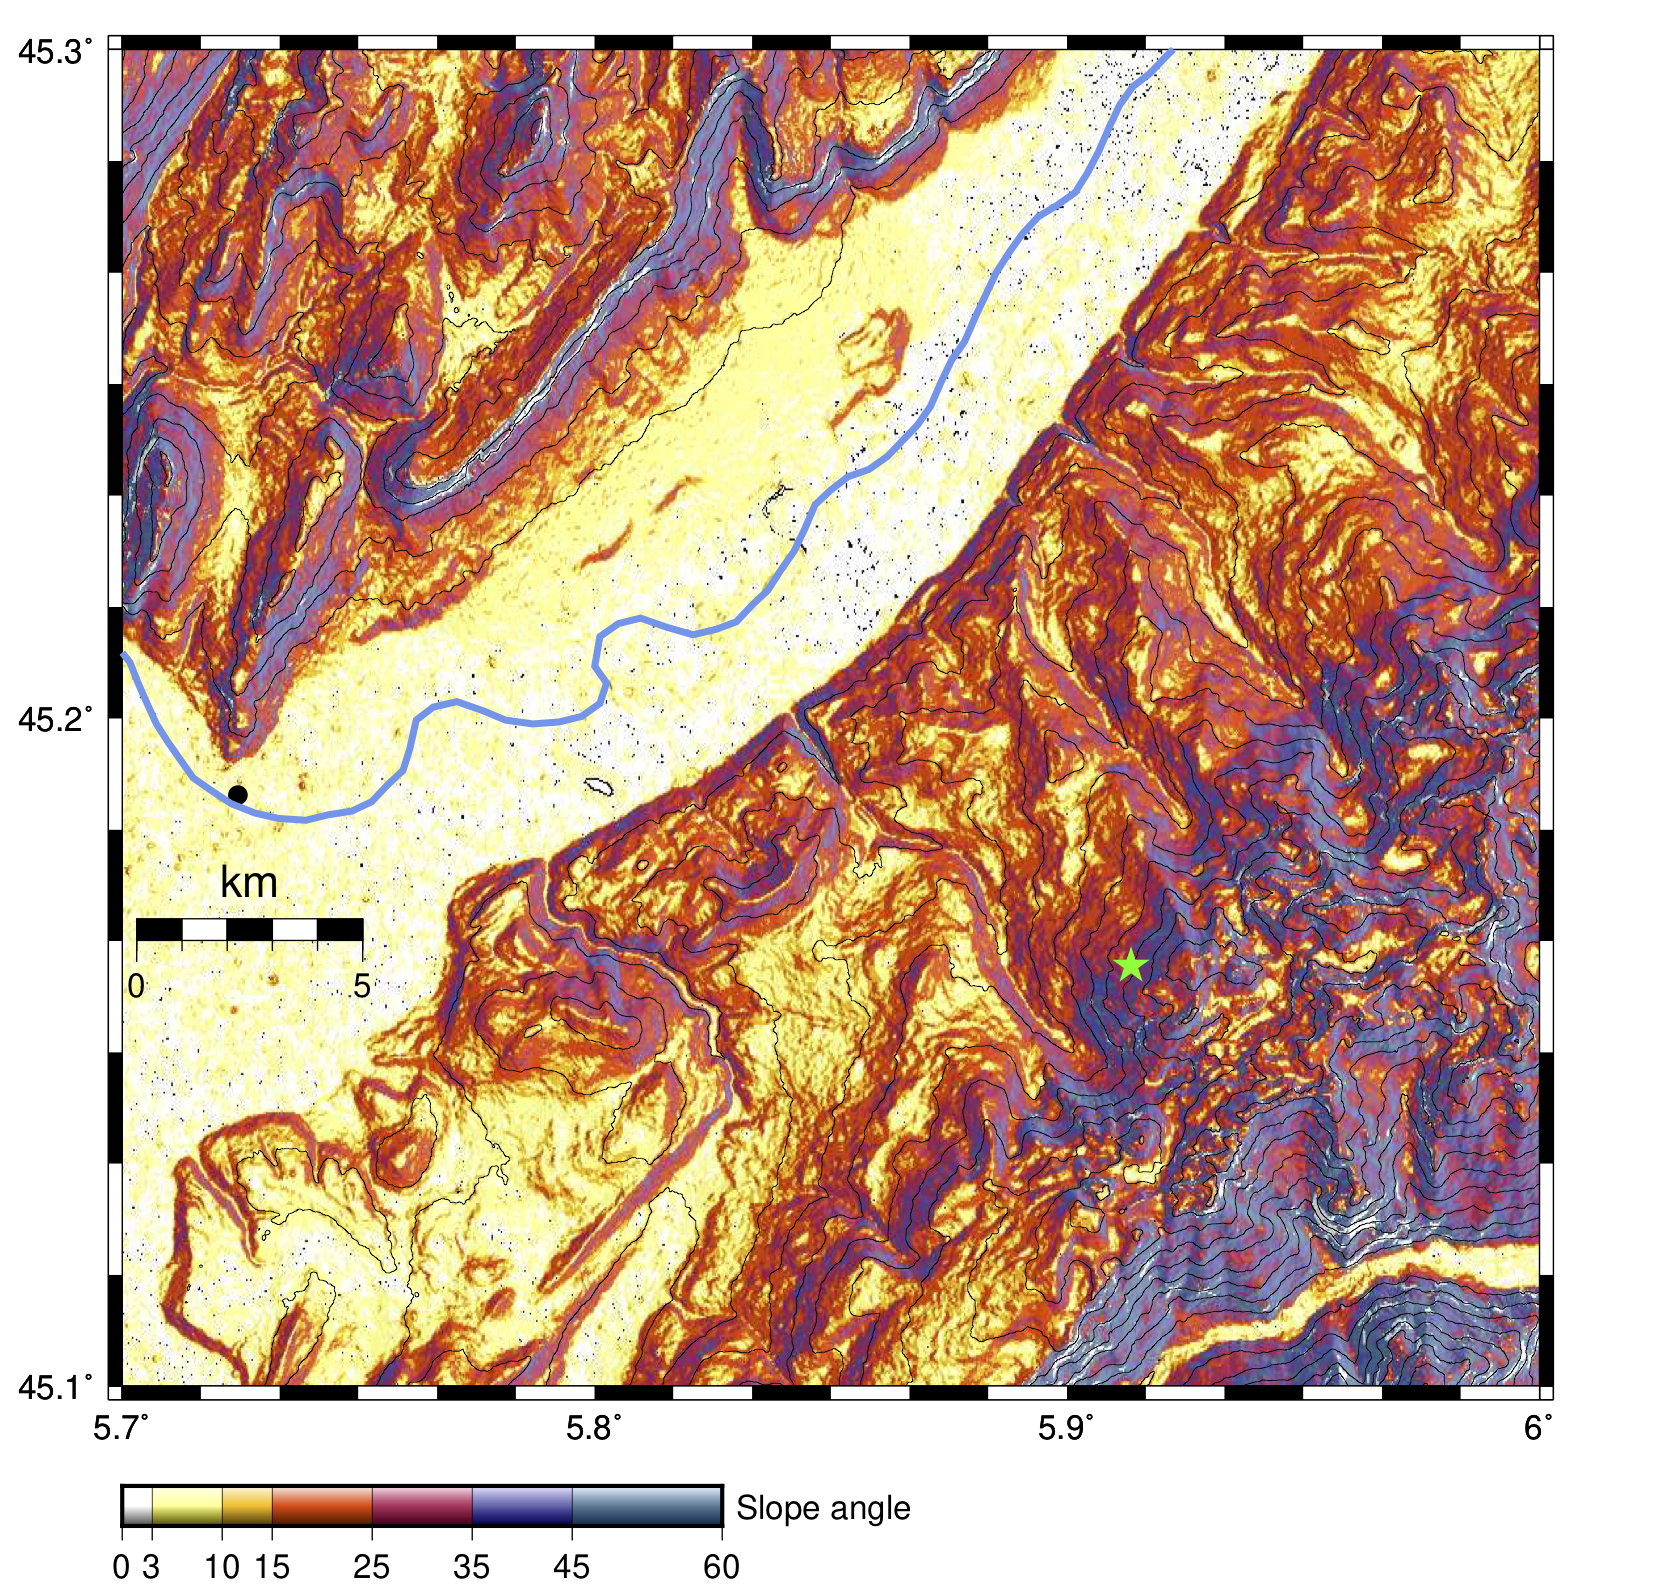
\includegraphics[width=0.8\textwidth]{fig/chapter_3/grenoble_slopes_C100.png}
  \caption{Topographic map showing the slopes of the region. The green star marks the position of the measuring site. The black dot marks the localisation of Grenoble. Data obtained from Shuttle Radar Topography Mission using the GMTSAR processing system~\citep{sandwell2011gmtsar}.}
  \label{fig:obs_site}
  \end{center}
\end{figure}

The meteorological station was located at 1770~m height, located in an alpine pasture area (low vegetation and sparse rocks or pebbles) above the forest area and
has a relatively homogeneous slope, which fulfils the essential characteristics for a detailed analysis of the physical process~\citep{blein2016observation}. In particular, the ground was covered by a layer of snow which thickness decreased during the field campaign. The average slope of the site is around 30~$\degree$.

\section{Instrumentation} \label{instrumentation}

The instruments placed in the field were mounted into two masts. The principal mast measured 10~m and on it were mounted 11 sonic anemometers and 10 thermocouples (see figure~\ref{fig:mast}). There was a smaller mast (2~m) with a meteorological station placed a few meters apart from the main mast. 

On the small mast, or meteorological mast, there were the following instruments installed: 
\begin{itemize}
    \item CS100 standard barometer (Campbell Scientific), for atmospheric pressure.
    \item CNR1 net radiometer sensor (Campbell Scientific), for short and long wavelength radiation fluxes.
    \item IR120 infrared radiometer (Campbell Scientific), for measuring the longwave radiation flux emitted by the ground.
    \item CS125 temperature and relative humidity sensor (Campbell Scientific).
    \item SR50 sonic ranging sensor (Campbell Scientific), for measuring the position of the sensors relative to the ground.
\end{itemize}

In the big mast there were four types of anemometers with different characteristics and only one type of thermocouple. The anemometers were the CSAT3 and CSAT3B~\footnote{The CSAT3B is the most recent version of the CSAT3.} 3-D sonic anemometers manufactured by Campbells Scientific, which measure three components of the wind with a frequency of 20~Hz. In total there were five CSAT3 and only one CSAT3B. Also, we used four Windsonic 2-D sonic anemometers manufactured by Gill Instruments. This anemometer measures two components of the mean wind that are aligned to the "plane" of the instrument. At the top of the mast, a Windmater Pro Sonic Anemometer (from Gill Instruments) was placed. As the CSAT3, it measured three components of the wind with a frequency of 20~Hz. The Table~\ref{tab:intruments_anemometers} shows the initial heights of the the anemometers.

\begin{table}[!ht]
    \centering
    \begin{tabular}{ | l | c | c | c |}
    \hline
    \textbf{Instrument} & \textbf{Variables measured} &  \textbf{Frequency (Hz)} & \textbf{Initial height (m)} \\ [0.5ex]  \hline\hline
    CSAT3B & \multirow{6}{*}{(u,v,w) and Temp.} & \multirow{6}{*}{20} & 0.035 \\
    CSAT3 No.5 &  &  & 0.36 \\
    CSAT3 No.4 &  &  & 0.67 \\
    CSAT3 No.3 &  &  & 1.16 \\
    CSAT3 No.2 &  &  & 1.57 \\
    CSAT3 No.1 &  &  & 1.98 \\
    \hline
    Windsonic 2D No.3 & \multirow{4}{*}{(u,v)} & \multirow{4}{*}{0.003} &  2.7\\
    Windsonic 2D No.2 &  &  &  3,69\\
    Windsonic 2D No.1 &  &  &  5.42\\
    Windsonic 2D No.0 &  &  &  7.02\\
    \hline
    Windmaster Pro & (u,v,w) and Temp. & 20 & 8.97 \\
    \hline
    
    \end{tabular}
    \caption{Specification for the different anemometers installed.}
    \label{tab:intruments_anemometers}
\end{table}

An important aspect of the anemometers is their orientation and alignment with respect to the slope. In this case, we aligned all the anemometers in a manner that the horizontal wind components of the instruments were parallel to the slope surface and the vertical wind component perpendicular to the surface (figure~\ref{fig:mast_pics} shows how the instruments are tilted, following the slope of the mountain). The orientation of the instruments was different for the CSAT3, the Windsonic 2-D and the Windmaster Pro. The CSAT3 and CSAT3B were oriented towards the south (180~$\degree$ North off-set), in a way that the $v$ component of the wind was facing the slope (eastwards) and the $u$ was facing the right side of the slope (southwards). The Windsonic 2-D was oriented towards the West (270~$\degree$ North off-set) in a manner that the negative $u$ component was facing the slope (facing the towards the valley, i.e. towards the West). And the Windmaster Pro was facing towards the slope or facing East (90~$\degree$ North off-set).

\begin{figure}[!ht]
  \begin{center}
  \includegraphics[width=0.6\textwidth]{fig/chapter_3/Montage.jpg}
  \caption{Scheme of the principal mast with the position and label of the instruments.}
  \label{fig:mast}
  \end{center}
\end{figure}

\begin{figure}[!ht]
    \centering
    \begin{subfigure}[b]{0.308\textwidth}
        \includegraphics[width=\textwidth]{fig/chapter_3/foto_1_small.jpg}
    \end{subfigure}
    \quad
    \begin{subfigure}[b]{0.4\textwidth}
        \includegraphics[width=\textwidth]{fig/chapter_3/foto_3_small.jpg}
    \end{subfigure}
    \caption{To the left, we can see a picture of the principal mast viewed from the side and at the back is possible to see the small mast. In the picture in the right we can see a zoom on the CSAT3 anemometers viewed from bellow.}
    \label{fig:mast_pics}
\end{figure}

Spread along the mast, there are ten thin thermocouples, that were used to measure the air temperature with a minimal intrusion at high frequency (20~Hz). The initial heights of these instruments are shown in table~\ref{tab:intruments_thermocouples} and can be seen in figure~\ref{fig:mast} at the left of the mast, opposite to the anemometers.

\begin{table}[!ht]
    \centering
    \begin{tabular}{ | l | c | c | c |}
    \hline
    \textbf{Instrument} & \textbf{Variables measured} & \textbf{Frequency (Hz)} & \textbf{Initial height (m)} \\ [0.5ex]  \hline\hline
    Thermocouple No.1 & \multirow{10}{*}{Temperature} & \multirow{10}{*}{20} &  0.05\\
    Thermocouple No.2 & &  &  0.13\\
    Thermocouple No.3 & &  &  0.21\\
    Thermocouple No.4 &  &  &  0.29\\
    Thermocouple No.5 & &  &  0.38\\
    Thermocouple No.6 &  &  &  0.47\\
    Thermocouple No.7 & &  &  2.53\\
    Thermocouple No.8 &  &  &  3.52\\
    Thermocouple No.9 &  &  &  5.26\\
    Thermocouple No.10 &  &  & 6.84 \\
    \hline
    
    \end{tabular}
    \caption{Specifications of the Thermocouples.}
    \label{tab:intruments_thermocouples}
\end{table}

%In the middle, there is a radiometer used to measure the radiant flux. Finally, there is an ultrasonic instrument installed in the station to record the height of the snow cover (snow-covered ground was expected in the measuring site). This is important because the snow decreases the height between the ground and the instruments, which is an important parameter in the calculations.

\section{Field campaign}

The field campaign could only take place during certain weather conditions and during winter. For this reason, we couldn't establish a certain date for it. First of all, winter is the season when the occurrence of katabatic winds event is greater because of the cold temperatures in the mountains. Also, the other important factor, as mentioned in section~\ref{sec:katabatic_winds}, is that the presence of mesoscale wind systems can overshadow or inhibit the formation of katabatic winds. For this reason, an ideal weather condition for measuring katabatic winds is during anticyclonic events, in which mesoscale wind systems are weak, the ski is clear and the air is cold.

During the month of February, between the 10th and the 28th,  Grenoble had anticyclonic weather conditions that were brought by three high-pressure systems that passed over the region during this period of time, these were named: Dorit, Erika and Frauke~\citep{highslist}. This meteorological window allowed us to carry out the field campaign. In total, the instruments took measurements for 17 days.

\section{Data processing}

In total around 11.5~GB were obtained during the campaign, only taking into account the anemometers, the thermocouples and the meteorological station. The processing of the data depended on the instrument and its frequency of operation. 

\subsubsection{CSAT3 and Windmaster Pro}

For the CSAT3 anemometers and the Windmaster Pro we used EddyPro, which is a software that uses the eddy covariance method to compute atmospheric fluxes of certain trace gases, heat flux and energy~\citep{burba2013eddy}. EddyPro computes the averages of each of the components of the wind and the temperature for a certain period of time which we choose. After this, it computes the fluctuations (turbulent parts) of the variables and computes the covariance between them. There are multiple choices for software that can do this but EddyPro integrates different functions and methods that improve the quality of the output. 

The raw data of the sonic anemometers is in ASCII format, which EddyPro can read only pointing out what are the columns corresponding to each variable and each instrument. For this also we have to specify the height of the instruments with respect to the ground, the orientation of the instruments with respect to the north, the type of average to compute and the period for computing the average. 

Due to the number of days the instruments were operating and the high frequency of acquisition, it was convenient to use a relatively large period for averaging to try to identify the days when there were good conditions for katabatic winds to form. For this reason, we processed the data doing 30 minutes averages for both the CSAT3 anemometers and the Windmaster Pro. This type of average works as a low-pass filter for the raw high-frequency signal, where all the turbulent fluctuations of the variables are lost. For this reason, is only convenient to use this 30~minutes averaged data to identify potential good periods with the required conditions and not to analyse the turbulent characteristics of the flow

After identifying three potentially good nights for katabatic winds episodes, we went back to EddyPro and processed the data using a 5~minutes average period, which works better to analyse the turbulent characteristics of the flow and the respective fluxes. In particular we computed the sensible heat flux ($\overline{w'\theta'}$), the momentum flux ($\overline{u'w'}$) and the turbulent kinematic energy (TKE).

\subsubsection{Thermocouples and Windsonic 2-D anemometers}

As mentioned before, the raw data of the thermocouples have a frequency of 20~Hz, and the Windsonic anemometers record 5~minutes-averages. Both instruments are incompatible with EddyPro because they do not measure wind velocity and temperature simultaneously, which makes them unfit for the eddy covariance method used by the software. This is why for these instruments it was necessary to write a script to compute the average at a different frequency. As with the 3-D sonic anemometers, first, we did a 30 minutes average of the data for both type of instruments, to be able to analyse and detect the best nights to observe katabatic wind. After determining the ideal nights, we performed 5~minute averages of the raw data.

\section{Temperature comparison between thermocouples and CSAT3 anemometers}

With the 30~minute averaged data, we compared the temperature measured by the CSAT3 instruments with respect to the temperature of the thermocouples. We did this to verify that the temperature of the sonic anemometers was consistent because this temperature is used to compute the heat fluxed, which is an important aspect of the flow. 

For this, we selected a thermocouple and a CSAT3 placed at the same height or very close in height to one another. From figure~\ref{fig:mast} and the tables~\ref{tab:intruments_anemometers}~and~\ref{tab:intruments_thermocouples} is possible to see that the CSAT3B and the Thermocouple No.1 are very close in height, only 1.5~cm of difference. Also, the CSAT3 No.5 and the Thermocouple No.5 are very close with 2~cm of difference. To this data, we did a calibration plot of the temperature of both instruments (CSAT3 vs Thermocouple) and computed the correlation coefficient. This gave us an insight into how well the measurements of temperature obtained from the CSAT3 are. 

\section{Wind speed comparison between CSAT3 and Windsonic 2D anemometers}

As in the previous section, and because we have three types of anemometers installed in the mast, it was necessary to check that the measurements of the wind speed were consistent between instruments. For this, we selected the closest CSAT3 to the WINDSONIC 2D no.3, which is the closest to the ground from the Windsonic's installed. The CSAT· No.1 is the closest one to this instrument, with a vertical separation of 72~cm. For this we only compared mean the wind speed of both instruments, disregarding the wind direction, and did a scatter plot for both instruments, computing the correlation coefficient. 

The comparison between the Windmaster Pro and the Windsonic 2-D was not performed because the separation between the closest Windsonic anemometer to the wind master on the top is of around 2~m. 

\section{Wind direction correction}

When analysing the wind direction data from all the anemometers we saw that there where inconsistencies with the wind direction of the CSAT3B anemometer, placed at the bottom of the mast. We found out that there was a systematic deviation of $+90\degree$ with respect to the other CSAT3 instruments, and the variation of the angle was inverted with respect to the other CSAT3's. To identify this we did a calibration plot (see appendix~\ref{app:wind_dir}) between the wind direction of the CSAT3B and the CSAT3 No.5, which is the closest one to the CSAT3B, and proposed a correction, which we implemented when analysing the data.

\section{Ground temperature calculation}

Using the data from the radiometer CNR1 installed in the small mast, in specific the longwave emitted radiation from the ground (considered as a black body), we computed the ground temperature using the Stephan-Boltzmann Law:

\begin{equation}
    I = \sigma T^4, 
\end{equation}

\noindent which relates the radiant emittance with respect to the temperature of a body, where $\sigma = 5.67 \times 10^{-8} W m^{-2} K^{-4}$, is the Stephan-Boltzmann, and $T$ is the body temperature. Solving for $T$ and using the longwave emitted radiation from the ground as $I$, we computed the time series of the temperature of the ground.

%With the ground temperature, we computed the temperature gradient between the ground and the CSAT3 No.4. We choose the CSAT3 No.4 because is placed in the middle of the CSAT3 array and is not to close to the ground. To compute the gradient we did the operation:

%\begin{equation}
%    \text{grad}_z T = \frac{T_{csat} - T_{grd}}{h_{csat} - h_{grd}},
%\end{equation}

%\noindent where $T_{csat}$ and $T_{grd}$ are the CSAT3 No.4 and ground temperature respectively at certain time. The height of both instruments are the variables $h_{csat}$ and $h_{grd}$ respectively. Because this height is measured with respect to the ground, $h_{grd} = 0$, and we use the corresponding value of the height of the CSAT3 No.4 at each particular time. 

\section{Criterion for choosing the nights to analyse}

The criteria for detecting katabatic winds can be summarized in two important aspects: Temperature gradient and external forcing. The temperature gradient refers to the vertical temperature gradient between the ground and the air. When there is a strong vertical gradient, where the ground is colder than the air above it, the gradient forms a stable stratification of the air. During the night is when the ground is colder because of the absence of incident solar radiation, which decreases the ground temperature, and therefore, starts to cool down the air that is in contact with, creating the conditions for the katabatic wind to form. For this reason, we restricted our analysis to the nights of the field campaign. 

The other aspect is that there should not be signs of externals forcing or strong winds blowing, which can inhibit the formation of the katabatic wind. A way to detect this is when the data suddenly registers peaks in the wind speed for all the different heights. Also, these external forcing have the characteristic of carrying hotter air compared with the ambient temperature of the air. This means that when the data displays sudden jumps in wind speed and air temperature, is due to an external weather system that is passing through the region, and the possibility of detecting katabatic flows is low.

The first filter used to detect the optimal nights was direct observation done during the campaign, where it was registered the atmospheric conditions and the intensity of the wind in the measuring site. This gave us an insight into the potentially good nights with low wind speeds and allow us to focus the analysis in them.

Finally, when these conditions are gathered, we should be able to see a maximum in the mean wind speed profile close to the ground, with a downslope wind. This is the signature of katabatic winds.

\section{Results}
As mentioned in the Methodology section~\ref{sec:methodology}, the first step was to analyse time series of the anemometers and thermocouples averaged in a 30 minute period. 

The top panel of figure~\ref{fig:temp_series} shows the CSAT3 air temperature and the ground temperature measurements. At first glance is possible to see that there is a gap in the data between the 17th and the 19th of February when none of the CSAT3 instruments were measuring. In the lower panel, we can see the time series of the Thermocouples. They follow a similar variation as the CSAT3 instruments, but they were recording during the whole campaign. 

\begin{sidewaysfigure}
  \centering
  {
  \includegraphics[width=1\textwidth]{fig/chapter_4/csat_temp_series.png}\\
   \includegraphics[width=1\textwidth]{fig/chapter_4/TC_temp_series.png}
   }
  \caption{Time series of air temperature of the whole field campaign. The top panel shows the air temperature recorded by the CSAT3 instruments and the lower panel the air temperature recorded with the Thermocouples. In both figures, the grey shadows represent the night periods, the green shadows the favourable days from in situ observation and the yellow shadows the nights chosen for the analysis. Both plots have the ground temperature as a reference point.}
  \label{fig:temp_series}
\end{sidewaysfigure}

In figure~\ref{fig:windspeed_series} the time series (30 minutes average) of the wind speed of the CSAT3 and the Windsonic anemometers are shown. The top panel corresponds to the CSAT3's, where is possible to see the gap of the data in the middle of the campaign. The lower panel corresponds to the Windsonic 2-D instruments, where we can see that during the beginning of the campaign (from the 12th to the 19th) only the Winsonic No.0 and No.1 were working. From the 19th until the end of the campaign, the four Windosinc were working. 

\begin{sidewaysfigure}
  \centering
  {
  \includegraphics[width=1\textwidth]{fig/chapter_4/wind_speed_csat_series.png} \\
   \includegraphics[width=1\textwidth]{fig/chapter_4/wind_speed_ws_series.png}
   }
  \caption{Time series of wind speed of the whole field campaign. The top panel shows the wind speed recorded by the CSAT3 instruments and the lower panel the winds speed recorded with the Windsonic 2-D (WS). In both figures, the grey shadows represent the night periods, the green shadows the favourable days from in situ observation and the yellow shadows the nights chosen for the analysis. Both plots have the ground temperature as a reference point.}
  \label{fig:windspeed_series}
\end{sidewaysfigure}

In both figures~\ref{fig:temp_series} and \ref{fig:windspeed_series}, there are periods marked by green and yellow shadows. The green ones indicate the favourable days for the development of katabatic winds, according to the in situ observations: cold nights with steady decrease of surface temperature during the night with weak wind. The yellow periods indicate the nights that were selected for the analysis in this work, according to the criteria for choosing a good night. We selected the nights of the 16th to the 17th and the night from the 23rd to the 24th. These were chosen because there was a pronounced drop in the temperature of the ground and the air and because they were in the favourable periods to detect these winds. 

For the 16-17th night, the instruments recorded a drop in the average temperature of more than $5\degree C$ for the ground temperature and air temperature, from the sunset until midnight. At midnight the instruments measured a small increase in the temperature of the air, which probably was caused by the presence of an external wind system. If we look at the wind speed profiles, on the same night, we can see that at the end of the afternoon the wind is relatively calm, and increases its intensity during the night. During the 23-24th night, the conditions were similar, with the exception that the ground and air temperature decreased very uniformly throughout that night.

\section{Calibration}

To corroborate that the measurements of temperature and wind speed done by different types of instruments where congruent between them, we performed some comparisons between the CSAT3's and the Thermocouples, for temperature, and the CSAT3's with the Windsonics, for the wind speed.

Figure~\ref{fig:csat1_vs_ws3} shows a scatter plot comparing 30 minutes averaged wind speed, measured with the Windsonic 2-D, versus the wind speed measured with the CSAT3-B. Using the data of the whole campaign, a linear regression was done, from which it was found a correlation coefficient $R = 0.94$. This means that both wind speeds are correlated and their variation in time is similar. 

\begin{figure}[!ht]
    \centering
    \includegraphics[width=0.48\textwidth]{fig/chapter_4/gunshot_csat1_vs_ws3.png}
    \caption{Scatter plot comparing the wind speeds of the Windsonic 4 and the CSAT3 No.1. The red line is a linear fit done to the data, with a correlation coefficient $R$ of 0.94.}
    \label{fig:csat1_vs_ws3}
\end{figure}

Figure~\ref{fig:csat_vs_TC} shows the comparison of the temperature measured with the CSAT3 and the Thermocouples. In particular, the figure on the left is the comparison between the CSAT3-B and the thermocouple 1, which are the instruments closest to the ground. It's correlation coefficient is $R = 0.996$. On the right side, the figure compares the CSAT3 No.4 with the Thermocouple 6. The data had a correlation coefficient $R = 0.989$. Thus the sensors seem reliable to measure the temperature.

In overall, the CSAT3 anemometers seem to perform good measurements of temperature compared to the Thermocouples and the Windsonic 2-D measurements are congruent with the wind speed measured by the CSAT3 anemometers.

\begin{figure}[!ht]
    \centering
    \begin{subfigure}[b]{0.48\textwidth}
        \includegraphics[width=\textwidth]{fig/chapter_4/csat3b_vs_T1.png}
      \label{fig:csat3b_vs_TC1}
    \end{subfigure}
    \quad
    \begin{subfigure}[b]{0.48\textwidth}
        \includegraphics[width=\textwidth]{fig/chapter_4/csat4_vs_T6.png}
        \label{fig:csat4_vs_TC6}
    \end{subfigure}
    \caption{Comparison between the sonic temperature measured with the CSAT3 instruments with a Thermocouple placed at the same vertical level. Each plot has a correlation coefficient, $R$.}
    \label{fig:csat_vs_TC}
\end{figure}

%\section{Temperature gradient}

%Pending (probably not going to put it).

\section{Temperature and wind speed vertical profiles}

For sake of simplicity and because the nights of the 16-17th and 23-24th are similar, in this section we present only the 23-24th night, leaving the results of the 16-17th night for the appendix~\ref{app:profiles}. 

%\subsection{Night of the 23th to the 24th}

\begin{figure}[!ht]
    \centering
    \includegraphics[width=1\textwidth]{fig/chapter_4/23-24/18-21_profiles.png}
    \caption{Temperature and wind speed vertical profiles, with the corresponding wind direction at a particular time, for the period between 18h00 and 20h30 on the night of the 23-24th.}
    \label{fig:18-21_profiles.png}
\end{figure}

Figure~\ref{fig:18-21_profiles.png} shows the vertical mean profiles of air temperature and wind speed over a period between 18h00 and 20h30. The air temperature profiles show the measurements done using the Thermocouples (T1 - T10). The wind speed profiles show the measurements done by the CSAT3 and Windsonic 2-D anemometers. At the right of the figure is possible to see a polar plot with the wind direction (point into the direction where the wind is coming to the instrument). The $0 \degree$ angle is aligned with the North. Each level of different radius corresponds to the value of a certain instrument: closer to the centre is the CSAT3-B (B), and in the outer radius, the Windsonic 2-D No.0 (WS0). Globally, the colour of the curves and points on the three subfigures correspond to the values at the same hour, which allows us to identify the temperature, the wind speed and the direction of the profile at a particular time.

\begin{figure}[!ht]
    \centering
    \includegraphics[width=1\textwidth]{fig/chapter_4/23-24/21-23_profiles.png}
    \caption{Temperature and wind speed vertical profiles, with the corresponding wind direction at a particular time, for the period between 21h00 and 23h30 on the night of the 23-24th.}
    \label{fig:21-23_profiles.png}
\end{figure}

Similar to the previous figure, figure~\ref{fig:21-23_profiles.png} shows the vertical profiles of air temperature and wind speed for the period between 21h00 and 23:30, with the corresponding wind direction.

The figures~\ref{fig:18-21_profiles.png} and \ref{fig:21-23_profiles.png} show typical profiles of katabatic wind, characterised by having a low
wind speed with a maximum close to the surface, inside a stable environment where temperature increases with height. Also, in the period shown in both figures, we can see a persistent wind direction coming from the downslope direction, especially in the lower levels. This confirms that during this night there were katabatic winds coming down the slope of the mountain. 

\section{Vertical fluxes and TKE}

In this section, we present the momentum flux ($\tau$), the sensible heat flux ($H$) and the Turbulent Kinematic Energy (TKE), computed with a five minutes average for the night of the 23-24th of February. As in the previous section, the fluxes for the night of the 16-17th can be found in the appendix~\ref{app:profiles}.

\begin{figure}[!ht]
    \centering
    \begin{subfigure}[b]{0.58\textwidth}
        \includegraphics[width=\textwidth]{fig/chapter_4/23-24/Tau_23-24.png}
      \label{fig:Tau_23-24}
    \end{subfigure}
    \begin{subfigure}[b]{0.58\textwidth}
        \includegraphics[width=\textwidth]{fig/chapter_4/23-24/H23-24.png}
        \label{fig:H_23-24}
    \end{subfigure}
    \begin{subfigure}[b]{0.58\textwidth}
        \includegraphics[width=\textwidth]{fig/chapter_4/23-24/TKE23-24.png}
        \label{fig:TKE_23-24}
    \end{subfigure}
    \caption{Time series of the momentum flux (upper figure), temperature flux (middle figure) and Turbulent Kinetic Energy (lower figure). }
    \label{fig:23-24_flux_series}
\end{figure}

Figure~\ref{fig:23-24_flux_series} shows the time series from the three fluxes between the 20h00 up to 23h30. These fluxes are only shown for the CSAT3 anemometers, and that is because these instruments measure simultaneously the temperature and the three components of the wind, making them the only anemometers to be able to compute these variables. The time series shows the variation of these quantities over time but is difficult to identify the value that corresponds to a particular instrument, for that it is useful to plot vertical profiles.

To improve the analysis we selected a particular hour, based on the 30 minutes average profiles, that had a clearly defined maximum wind speed and with a wind direction coming from $90\degree$ upslope. With this in mind, we selected two hours during the night and plotted the vertical profiles. The selected times were 20h00 and 23h00. Figure~\ref{fig:vert_prof_a} shows four profiles around 20h00, where at the left is the momentum flux ($\tau$), the second panel corresponds to the sensible heat flux ($H$), the third is the Turbulent Kinetic Energy (TKE) and the fourth one is the wind speed profile ($u$). In the same manner, figure~\ref{fig:vert_prof_b} shows the profiles for the fluxes, the TKE and the wind speed around 23h00. 

\begin{figure}
    \centering
    \includegraphics[width=1\textwidth]{fig/chapter_4/23-24/vert_prof_a_speedmax.png}
    \caption{Vertical profiles of momentum flux ($\tau$), sensible heat flux ($H$), Turbulent Kinetic Energy (TKE) and wind speed ($u$), for the night of the 23-24th of February, around 23h00.}
    \label{fig:vert_prof_a}
\end{figure}

Figure~\ref{fig:vert_prof_a} shows that the wind speed maximum is located at the same level as the CSAT3 No. 5, i.e. between 0.5m and 0.75m. In theory, the momentum flux at the maximum has to be equal to zero, which is the case of the profile corresponding to 20h10. For the other profiles, we see that the zero in the momentum flux is higher, at 1m or more. And at 19h55, we see that the momentum flux is always negative. As well, we can see that $\tau$ is strong in magnitude close to the surface due to strong shear stress caused by friction. 

\begin{figure}[!ht]
    \centering
    \includegraphics[width=1\textwidth]{fig/chapter_4/23-24/vert_prof_b_speedmax.png}
    \caption{Vertical profiles of momentum flux ($\tau$), sensible heat flux ($H$), Turbulent Kinetic Energy (TKE) and wind speed ($u$), for the night of the 23-24th of February, around 23h00.}
    \label{fig:vert_prof_b}
\end{figure}

Regarding the sensible heat flux ($H$) on figure~\ref{fig:vert_prof_a}, we see that it is always negative for all the profiles. This is due to the stable environment where the air is colder in the lower layers. The vertical profiles were expected to be constant with height, but the profiles show variations, which are difficult to explain. Concerning the Turbulent Kinetic Energy, it is small close to the surface due to the strong stability of the layer because is related to a strong temperature gradient. In the upper levels, the TKE is large due to the large shear stress and a smaller temperature gradient.

Finally, figure~\ref{fig:vert_prof_b} shows the vertical profiles corresponding to 23h00. In a similar way than the previous figure, The mean wind maximum is located at the level of the CSAT3 No.5. The momentum flux is negative for the lower part of the profile, below the maximum, and is positive above the maximum. The Sensible heat flux remains negative as expected (stable profile), but there are still some variations that are difficult to explain. For the TKE, we see that the profiles are similar to the ones in figures~\ref{fig:vert_prof_a}, with the lower value at the lower layer, and a larger one above the wind maximum.

\section{Conclusion}
The calibration done between the different type instruments showed that there was consistency between the temperature of the Thermocouples and the CSAT3's, measured at similar heights. Although, there was a significant horizontal separation between the CSAT3-B and the Thermocouple No.1 and between the CSAT3 No.4 and the Thermocouple No.4, the measurements where similar, as the high correlation value pointed out. This gave us the confidence of using the measurements of the Thermocouples to characterise the vertical profiles, with the advantage that there were more Thermocouples installed on the mast that CSAT3's to measure the temperature.

Doing the same calibration between the wind speed measured with the lowest Windsonic 2-D and the highest CSAT3, we found that the correlation was of 0.94, which shows that the wind speed of both instruments had the approximate same magnitude, even though there was a vertical separation of 0.7m between them. This is important at the moment of plotting the mean vertical wind profiles because there must be coherence in the measurements done with a different type of instruments for the profile to make sense. 

From the whole campaign, we were able to identify two nights with katabatic winds. As shown by the vertical profiles, the maximum in the mean wind speed was located between 0.5~m and 0.75~m. We expected to find this maximum at a higher level, to have two CSAT3's that could measure the wind below the maximum and two CSAT3's above the maximum, but instead of this, only one anemometer measured the wind below the maximum. 

During the night of the 23rd to the 24th, the momentum fluxes profiles showed a negative flux for the levels below the wind maximum and a positive flux above the maximum, with the exception of some rogue profiles that were negative at all levels or were negative above the wind maximum. Regarding the sensible heat flux, all the profiles were negative because of the stable environment, but there where some variations when the profiles should remain constant. For the TKE, the profiles showed a small value of TKE close to the surface, and an increase of TKE as the height increased, which correspond to what was expected. 

Globally, the campaign was a success because of the 17 days of anticyclonic conditions, which allowed to take sufficient measurements of katabatic winds structure, with better spacial resolution due to the improvements implemented based on previous campaigns. Despite that this work focused only on two nights, there are still many other nights to analyse and a lot of work ahead to do.

\clearpage
%\medskip
%\nocite{*}
\bibliographystyle{apalike}
\bibliography{biblio}
%\printbibliography

\end{document}
